\documentclass{article}
\usepackage[UTF8]{ctex}
\usepackage{amsfonts}
\usepackage{amsmath}
\usepackage{float}
\usepackage{graphicx}
\usepackage{url}

\newcommand{\Bezier}{B\'ezier}

\usepackage{color}

% paragraph
\setlength{\parindent}{0pt}
\setlength\parskip{\baselineskip}
\renewcommand{\baselinestretch}{1.2}

\begin{document}

% 标题
\title{《计算机辅助几何设计》作业}
\author{ID号: 01  \qquad  姓名: 张三}  %递交作业时填上ID号和姓名
\date{2021年10月12日}
\maketitle


1. 证明:一条空间\Bezier 曲线为平面曲线的充要条件是其控制顶点共面。

2. 证明:一条\Bezier 曲线的弧长不大于其控制多边形的周长。

3. 证明:圆弧不能用\Bezier 曲线精确表示。

4. 试求平面$n$次\Bezier 曲线及其控制顶点首末顶点与原点所围成的区域(如下图灰色区域)的面积(用控制顶点的坐标来表达)。
\begin{figure}[H]
  \centering
  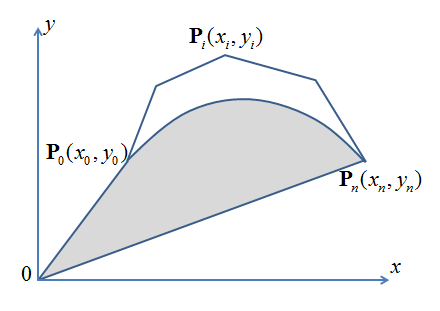
\includegraphics[width=0.4\textwidth]{fig-1}\\
  \label{fig:fig-1}
\end{figure}

5. 编写程序实现使用\Bezier 曲线来拟合平面点列。


{\color{blue} \bf{作业要求}}

学习使用LaTeX来编辑数学文档(未来写研究论文都要使用LaTeX来写),只要根据LaTeX模板修改来写,不必什么都学。并使用TeX/LaTeX来完成本次作业.

1) 请统一使用LaTeX的模板,可从以下链接下载:\\
\url{http://staff.ustc.edu.cn/~renjiec/tex-sample.zip} \\
2) TeX安装软件(最新版已含中文支持):\\
https://miktex.org \\
3) 有关TeX的学习教程或资料:\\
https://pan.baidu.com/s/1pLr5q2J

\end{document}
